\let\texyear\year
\documentclass{ieeeaccess}
\let\ieeeaccessyear\year
\let\year\texyear

\usepackage{cite}
\usepackage{amsmath,amssymb,amsfonts,mathtools}
\usepackage{amsthm}
\usepackage{algorithmic}
\usepackage{graphicx}
\usepackage{textcomp}
\usepackage{booktabs}
\usepackage{array}
\usepackage{enumitem}
\usepackage{xcolor}
\usepackage{url}
\usepackage{xspace}
\usepackage{comment}
\usepackage{tikz}
\usepackage{float}
\usepackage[caption=false]{subfig}
\usepackage{expl3}
\usepackage{xparse}
\usepackage{xr}
\externaldocument[main-]{paper2}
\usetikzlibrary{arrows.meta,shapes,automata,positioning,calc,fit,tikzmark,decorations.pathreplacing,decorations.markings}
% Unified monochrome figure style for the paper.
% All automata and timing diagrams use white states, black borders and black arrows.
\tikzset{
  fmstate/.style={
    circle, draw=black, fill=white, line width=0.6pt,
    minimum size=9mm, inner sep=1pt, font=\small
  },
  fmstatewide/.style={
    rounded rectangle, draw=black, fill=white, line width=0.6pt,
    minimum height=8mm, inner xsep=3pt, inner ysep=1.5pt, font=\small
  },
  fmaccept/.style={fmstate,double,double distance=1.2pt},
  fmerror/.style={fmstate,double,double distance=1.2pt,fill=gray!12},
  fmedge/.style={->,>=Stealth,line width=0.6pt},
  fmlabel/.style={font=\scriptsize,align=center,fill=white,inner sep=1.2pt},
  fminvariant/.style={font=\scriptsize,align=center},
  fmnote/.style={font=\scriptsize,align=center},
  fmtimeline/.style={->,>=Stealth,line width=0.6pt},
  fmevent/.style={circle,draw=black,fill=white,line width=0.6pt,minimum size=4.5mm,inner sep=0.5pt},
  fmreference/.style={fmevent,double,double distance=0.8pt},
  fmguide/.style={densely dashed,line width=0.45pt},
  fmbrace/.style={decorate,decoration={brace,amplitude=4pt},line width=0.5pt}
}


\providecommand{\Nat}{\mathbb{N}}
\providecommand{\Real}{\mathbb{R}}
\providecommand{\CVal}{\mathsf{val}}
\providecommand{\T}{\mathcal{T}}
\providecommand{\Val}{\mathsf{val}}
\providecommand{\Inv}{\mathit{Inv}}
\providecommand{\optimize}{\mathsf{optimize}}
\providecommand{\export}{\mathsf{export}}
\providecommand{\hUntil}{\mathbin{\widehat{\mathsf U}}}
\providecommand{\hRelease}{\mathbin{\widehat{\mathsf R}}}
\providecommand{\hEventually}{\widehat{\Diamond}}
\providecommand{\hAlways}{\widehat{\Box}}
\newtheorem{theorem}{Theorem}[section]
\newtheorem{lemma}[theorem]{Lemma}
\newtheorem{proposition}[theorem]{Proposition}
\newtheorem{corollary}[theorem]{Corollary}
\newtheorem{assumption}[theorem]{Assumption}
\newtheorem{definition}[theorem]{Definition}
\bibliographystyle{IEEEtran}
\let\year\ieeeaccessyear
\renewcommand{\thesection}{S\arabic{section}}
\renewcommand{\thefigure}{S\arabic{figure}}
\renewcommand{\thetable}{S\arabic{table}}
\renewcommand{\theequation}{S\arabic{equation}}

\begin{document}
\history{}
\doi{}
\title{Supplementary Material for the Article: Mechanically Verified Optimization and UPPAAL Export for Timed B\"uchi Automata}
\author{\uppercase{Elie Fares}\authorrefmark{1},
\uppercase{Jean-Paul Bodeveix}\authorrefmark{2},
\uppercase{Hussain Al-Aqrabi}\authorrefmark{1} AND
\uppercase{Azar Salami}\authorrefmark{1}}
\address[1]{Higher Colleges of Technology, Sharjah, United Arab Emirates (e-mail: efares@hct.ac.ae, halaqrabi@hct.ac.ae, asalami@hct.ac.ae)}
\address[2]{IRIT, UPS, Universit\'e de Toulouse, France (e-mail: bodeveix@irit.fr)}
\begin{abstract}
This supplement gives detailed definitions and proof arguments for the verified TBA optimization and UPPAAL export passes, the full benchmark data and formula list, additional implementation checks, and the system models used in the UPPAAL case study. The Coq preservation results quantify over arbitrary TBAs; measurements are limited to benchmark automata recorded in the project.
\end{abstract}
\titlepgskip=-15pt
\maketitle
\section{The Verified Post-Processing Passes}
\label{sec:supp-passes}
This section details the passes summarized in Table~\ref{main-tab:post-passes} of
the article.

\subsection{Location Invariants on the Trace Model}
\label{sec:inv-semantics}
A location invariant maps every clock $x$ either to an upper bound
$M\in\mathbb R$, standing for the constraint $x\le M$, or to $+\infty$ (no
constraint).  We interpret automata with invariants on the extended words of
Section~\ref{main-sec:model}, as we do for automata without invariants.
Along a run $r$, the automaton stays in location $r(i)$ between the events
$i-1$ and $i$, and the invariant of $r(i)$ must hold during the whole stay,
that is, at the clock values $\CVal_\rho(i,x)-\tau$ for every delay
$\tau\in[0,\Delta_{i-1}]$, where $\Delta_{i-1}=t_i-t_{i-1}$ (and at the values $\CVal_\rho(0,x)$ for the
initial location).  This is the condition of Section~\ref{main-sec:model}, read at
the event that ends the stay.  Since clocks increase while time elapses, an
invariant made of upper bounds holds during the stay if and only if it holds at
the event that ends it (lemma \texttt{inv\_\allowbreak{}during\_\allowbreak{}iff\_\allowbreak{}at\_\allowbreak{}event}).
For the two-sided invariants of Section~\ref{sec:forward}, a lower bound
$x\ge m$ must likewise hold during the whole stay, hence at its beginning.

\subsection{Invariant Synthesis and Backward Propagation}
\label{sec:uppaal-invariants}
In the exported timed automaton, upper-bounded guards need invariants so that
time does not elapse past all useful outgoing transitions.  We compute location
invariants from outgoing upper bounds and propagate successor requirements
backward, following the standard timed-automata intuition of propagating
admissible time domains~\cite{[BGD04]}.

\paragraph{Upper bound of a guard.}
For a conjunctive guard $g$ and a clock $x$, let $\mathit{ub}_x(g)$ be the
smallest bound $m$ of the constraints $x\le m$, $x<m$, and $x=m$ occurring in
$g$, and $+\infty$ if $g$ contains none.  Other constraints are ignored.  A
valuation satisfying $g$ satisfies $x\le\mathit{ub}_x(g)$.

\paragraph{Invariant synthesis.}
For a location $\ell$ with outgoing transitions
$\ell\xrightarrow{g_i,Z_i}\ell_i$, $i=1,\dots,m$, the synthesized invariant is
\[
  \mathit{Inv}(\ell)(x)=\max_{1\le i\le m}\mathit{ub}_x(g_i),
\]
with $\mathit{Inv}(\ell)(x)=+\infty$ when $\ell$ has no outgoing transition.
Thus a clock that some outgoing guard does not bound does not appear in the
invariant.  The bound is always non-strict, even when it comes from a strict
guard $x<m$: the invariant only needs to be implied by the guard of the next
transition, and strictness is kept in the guards themselves.

\begin{theorem}[Invariant synthesis]
\label{thm:inv-synthesis}
For every TBA $\mathcal A$, the automaton $\mathcal A$ with the synthesized
invariants accepts the same timed words as $\mathcal A$.
\end{theorem}

\begin{proof}
Adding invariants can only remove runs.  Conversely, let $r$ be an accepting
run on $\rho$.  At every event $i$, the transition taken from $r(i)$ is enabled,
so its guard holds at the values $\CVal_\rho(i,x)$, which are therefore at most
$\mathit{Inv}(r(i))(x)$.  By the lemma \texttt{inv\_\allowbreak{}during\_\allowbreak{}iff\_\allowbreak{}at\_\allowbreak{}event}, the invariant of $r(i)$ holds during
the whole stay.  (Coq: \texttt{add\_\allowbreak{}invariants\_\allowbreak{}correct}.)
\end{proof}

\paragraph{Backward propagation.}
One propagation step strengthens every transition
$\ell\xrightarrow{g,Z}\ell'$ with the invariant of its target after the
resets:
\[
  g := g\wedge\mathit{Inv}(\ell')[Z:=0],
\]
where $\mathit{Inv}(\ell')[Z:=0]$ replaces every bound $x\le M$ on a reset clock
$x\in Z$ by the constant constraint $0\le M$, that is, by $\top$ if $M\ge0$ and
by $\bot$ otherwise.  Invariants are then synthesized again from the
strengthened guards.

\begin{theorem}[Backward propagation]
\label{thm:propagation}
For every TBA $\mathcal A$ and every $n\in\mathbb N$, the automaton obtained by
$n$ propagation steps accepts the same timed words as $\mathcal A$.
\end{theorem}

\begin{proof}
Strengthening guards can only remove runs.  Conversely, consider an accepting
run that takes $\ell\xrightarrow{g,Z}\ell'$ at event $i$ and then a transition
$\ell'\xrightarrow{g',Z'}\ell''$ at event $i+1$.  The second guard holds at event
$i+1$, so the values at that event are bounded by $\mathit{Inv}(\ell')$.  Clock
consistency gives $\CVal_\rho(i+1,x)=\Delta_i$ for $x\in Z$ and
$\CVal_\rho(i+1,x)=\CVal_\rho(i,x)+\Delta_i\ge\CVal_\rho(i,x)$ otherwise; hence
the strengthened guard $g\wedge\mathit{Inv}(\ell')[Z:=0]$ holds at event $i$.
The argument uses clock consistency, so the theorem is stated on timed words.
(Coq: \texttt{propagate\_\allowbreak{}accepts} and
\texttt{propagate\_\allowbreak{}n\_\allowbreak{}accepts}.)
\end{proof}

Each round of the optimization pipeline of Section~\ref{main-sec:main-pipeline}
applies one propagation step.  The tool repeats the rounds until the
automaton is structurally equal to the previous one, as an OCaml value, or
until 50 rounds have been performed; the bound guarantees termination, and the
theorem holds for every number of steps, whether or not a fixpoint is
reached.  On our benchmarks, the rounds reach a fixpoint after at most five
rounds.
The invariant computation at one location is summarized in the article's
Figure~\ref{main-fig:main-inv-unified}.

\paragraph{Example.}
We illustrate the algorithm on the automaton of Fig.~\ref{fig:inv-example},
which contains a two-location cycle $\ell_1\to\ell_2\to\ell_1$ and a self-loop
at $\ell_2$.  It has one clock $x$, the initial location $\ell_0$, and the
transitions
\[
\begin{aligned}
&\ell_0 \xrightarrow{a,\;Z=\{x\}} \ell_1,\quad
 \ell_1 \xrightarrow{b,\;x\le 2,\;Z=\emptyset} \ell_2,\\
&\ell_2 \xrightarrow{c,\;\top,\;Z=\emptyset} \ell_1,\quad
 \ell_2 \xrightarrow{d,\;x\le 1,\;Z=\emptyset} \ell_2.
\end{aligned}
\]
The edge $\ell_1\xrightarrow{b}\ell_2$ requires $x\le2$, and the self-loop at
$\ell_2$ requires the tighter bound $x\le1$.

\begin{figure}[t]
\centering
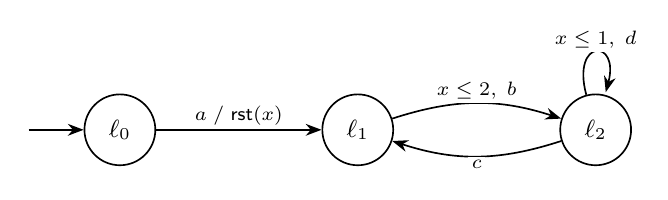
\begin{tikzpicture}[node distance=21mm]
  \node[fmstate] (l0) {$\ell_0$};
  \node[fmstate,right=of l0] (l1) {$\ell_1$};
  \node[fmstate,right=of l1] (l2) {$\ell_2$};
  \draw[fmedge] ([xshift=-7mm]l0.west) -- (l0.west);
  \draw[fmedge] (l0) -- node[fmlabel,above] {$a\;/\;\mathsf{rst}(x)$} (l1);
  \draw[fmedge] (l1) to[bend left=18] node[fmlabel,above] {$x\le2,\;b$} (l2);
  \draw[fmedge] (l2) to[bend left=18] node[fmlabel,below] {$c$} (l1);
  \draw[fmedge] (l2) edge[loop above] node[fmlabel] {$x\le1,\;d$} (l2);
\end{tikzpicture}

\caption{Automaton used to illustrate invariant propagation, with one clock $x$
and actions $a$--$d$.  Edges are labeled ``guard, action / resets'' (the guard
is omitted when it is $\top$); only the edge $\ell_0\to\ell_1$ resets $x$.  The
incoming arrow marks the initial location; acceptance plays no role here.  The
computed fixpoint is $\mathit{Inv}(\ell_1)=\mathit{Inv}(\ell_2)=(x\le2)$.}
\label{fig:inv-example}
\end{figure}

\begin{enumerate}
\item \emph{Synthesis.}  $\mathit{Inv}(\ell_1)(x)=\mathit{ub}_x(x\le2)=2$.  At
$\ell_2$, $\mathit{Inv}(\ell_2)(x)=\max(1,+\infty)=+\infty$, because the
transition toward $\ell_1$ does not bound $x$.  At $\ell_0$, the only outgoing
guard is $\top$, so $\mathit{Inv}(\ell_0)(x)=+\infty$.

\item \emph{Propagation.}  The transition
$\ell_2\xrightarrow{c,\;Z=\emptyset}\ell_1$ becomes guarded by
$\top\wedge\mathit{Inv}(\ell_1)=(x\le2)$.  The transition
$\ell_0\xrightarrow{a,\;Z=\{x\}}\ell_1$ receives $(0\le2)\equiv\top$ and is
unchanged.

\item \emph{Synthesis.}  At $\ell_2$, the outgoing guards are now $x\le1$ and
$x\le2$, so $\mathit{Inv}(\ell_2)(x)=\max(1,2)=2$.

\item \emph{Propagation.}  The transition $\ell_1\xrightarrow{b,\;x\le2}\ell_2$
receives $x\le2$, which it already contains, and the self-loop at $\ell_2$
receives $x\le2$, which is implied by $x\le1$.  Nothing changes.
\end{enumerate}
The fixpoint is $\mathit{Inv}(\ell_0)=\top$ and
$\mathit{Inv}(\ell_1)=\mathit{Inv}(\ell_2)=(x\le2)$.  While the automaton
remains in the cycle $\ell_1\leftrightarrow\ell_2$, the clock $x$ cannot exceed
$2$, and at every reachable valuation at least one outgoing transition of the
current location is enabled.  The invariants do not remove every blocking
behavior: since $x$ is never reset in the cycle, time is blocked once $x=2$.
They make the upper bounds of the property automaton explicit, and
Theorems~\ref{thm:inv-synthesis} and~\ref{thm:propagation} guarantee that they
do not change its language.

\subsection{Forward Propagation of Lower Bounds and Simplification}
\label{sec:forward}
\paragraph{Entry bounds.}
Dually, for a transition $t=\ell\xrightarrow{g,Z}\ell'$ and a clock $x$, the
\emph{entry bound} of $x$ along $t$ is $0$ if $x\in Z$ and otherwise the
largest bound $\mathit{lb}_x(g)$ of the constraints $x\ge m$, $x>m$, and $x=m$
of $g$, if any.  The entry bound of $x$ at a location $\ell'$ is the minimum of
the entry bounds of $x$ along the transitions entering $\ell'$; for the initial
location, the initial entry, with bound $0$, also counts.  If some entering
transition gives no bound on $x$, the clock $x$ has no entry bound at $\ell'$.
Since clocks are nonnegative and do not decrease while time elapses, every
clock with entry bound $m$ at $\ell'$ satisfies $x\ge m$ during every stay in
$\ell'$.

\paragraph{Forward propagation.}
The forward step adds $x\ge m$ to the guard of every transition leaving
$\ell'$, for every clock $x$ with entry bound $m$ at $\ell'$ (Coq:
\texttt{forward\_\allowbreak{}accepts}).  The entry bounds can also be read as lower-bound
invariants: the two-sided automaton that carries the synthesized upper-bound
invariants and the entry bounds as lower-bound invariants accepts the same
timed words (\texttt{add\_\allowbreak{}two\_\allowbreak{}sided\_\allowbreak{}invariants\_\allowbreak{}accepts}).  UPPAAL
rejects lower-bound invariants, and their only role is to make infeasible
transitions visible: after forward and backward propagation, a transition whose
source location bounds a clock from below and whose target bounds it from above
carries both bounds in its guard.

\paragraph{Simplification.}
Three simplifications follow.  First, a transition whose guard contains
contradictory constraints is removed: a lower bound and an upper bound on the
same clock with $u<l$, or with $u=l$ and one of them strict, or an upper bound
$x\le u$ with $u<0$ or $x<u$ with $u\le0$.  Such a transition is never enabled (Coq:
\texttt{remove\_\allowbreak{}contradictory\_\allowbreak{}accepts}).  Second, the transitions
leaving a non-initial location that has no entering transition
are removed: such a location never occurs on a run after position~$0$ (Coq:
\texttt{remove\_\allowbreak{}unreachable\_\allowbreak{}accepts}).  The iteration of the pipeline
removes chains of such locations one step at a time.  A location whose only
entering transitions are self-loops keeps them, but it is unreachable from
the initial location; the tool counts and prints only the locations
reachable from the initial one and their transitions.  Third, a transition whose
action label is unsatisfiable, because it requires two different actions or an
action and its negation, is removed (Coq:
\texttt{remove\_\allowbreak{}unsat\_\allowbreak{}accepts}).  Such labels arise because the
translator treats an action $a$ and the atom $\neg a$ of $\T(f)$ as independent
propositions; removing them also enables clock merging, since the resets of a
transition that can never be taken would otherwise prevent it.

\subsection{Dead Resets and Merging of Synchronously Reset Clocks}
\label{sec:dead-merge}
\paragraph{Dead resets.}
A clock $x$ is \emph{live} at a location $\ell$ if some transition that tests
$x$ in its guard can be taken from $\ell$, possibly after other transitions.
The live locations are computed as a backward closure, along all
transitions, from the sources of the transitions that test $x$; the other
locations are \emph{dead} for $x$.  Since the correctness of the pass does
not depend on how this closure is computed, the pass checks the two
properties that the proof uses, namely that no transition leads from a dead
location to a live one and that none tests $x$ from a dead location, and then removes $x$ from the reset sets of the
transitions that enter a dead location.  After such a transition, the value of
$x$ is never read again, so whether it is reset does not matter.  The proof
builds, from every accepted extended word, an extended word that differs only
in the reset decisions of $x$, and conversely (Coq:
\texttt{remove\_\allowbreak{}dead\_\allowbreak{}resets\_\allowbreak{}clock\_\allowbreak{}accepts}).  The pass is applied
to every clock (\texttt{remove\_\allowbreak{}dead\_\allowbreak{}resets\_\allowbreak{}accepts}).

\paragraph{Synchronous clocks.}
The verified translation shares the clock of syntactically identical timed
subformulas.  Clocks of \emph{different} subformulas can also be merged when
they are reset synchronously.  Two clocks $x\neq y$ are \emph{mergeable} if
\begin{enumerate}[label=(\roman*)]
  \item every transition resets $x$ if and only if it resets $y$;
  \item no transition enters the initial location; and
  \item every transition leaving the initial location resets $x$ and does not
        test it.
\end{enumerate}
Then, after the first event, $x$ and $y$ always have the same value, and every
test of $x$ can be replaced by the same test on $y$ (Coq:
\texttt{merge\_\allowbreak{}accepts}).  The condition is checked by a Boolean function
proved to imply it, and the pass tries all pairs of reset clocks
(\texttt{merge\_\allowbreak{}all\_\allowbreak{}accepts}).  The merged clock $x$ is no longer tested,
so its remaining resets are removed by the dead-reset pass in the next round.
This verified merging is restricted to synchronously reset clocks; merging
clocks whose values coincide for other reasons is not covered.

\subsection{Normalization of Guards}
\label{sec:normalize}
Backward and forward propagation add constraints to guards.  Every time a
guard is strengthened, it is \emph{tightened}: a constraint implied by another
constraint of the same guard on the same clock is dropped, so that a guard
keeps at most one lower bound and one upper bound per clock (an equality
counting as both); for instance, $x\le5\land x<2$ becomes $x<2$.  The
implication test compares bounds and strictness, and is proved sound (Coq:
\texttt{tighten\_\allowbreak{}holds}).  Normalization tightens every guard and also
removes the lower bounds $x\ge m$ with $m\le0$ and $x>m$ with $m<0$, which every
clock value satisfies; it is needed after the merging of clocks, which renames
constraints.  The removal of trivial lower bounds relies on the nonnegativity
of clock values, so the theorem is stated on timed words (Coq:
\texttt{normalize\_\allowbreak{}accepts}).

\subsection{Merging of Transitions and of Locations}
\label{sec:merge-ts}
\paragraph{Transitions.}
Two transitions with the same source, target, and resets are merged when the
union of their enabling conditions is again a conjunction.  A transition is
removed when another transition with the same source, target, and resets is
\emph{weaker}, that is, when its label and guard imply those of the other
transition, constraint by constraint (subsumption).  Two transitions
whose labels, or guards, differ only by a literal and its negation, such as
$p$ and $\neg p$, $x<2$ and $x\ge2$, or $x\le5$ and $x>5$, are replaced by one
transition without that literal (resolution).  The pass preserves the language
because every enabled transition has an enabled counterpart with the same
source and target, and conversely (Coq: \texttt{merge\_\allowbreak{}trans\_\allowbreak{}accepts}).
The other unions are disjunctive; they are formed by the export
(Section~\ref{subsec:disjunctive-invariants}).

\paragraph{Locations.}
A location $\ell'$ is merged into a location $\ell$ when both are accepting or
both are not, and when every transition leaving $\ell'$ has a twin leaving
$\ell$, and conversely: same label, guard, and resets, compared as sets, and
same target once $\ell'$ is replaced by $\ell$.  The transitions entering
$\ell'$ are redirected to $\ell$, and those leaving $\ell'$ are removed.  A run
of the original automaton becomes a run of the merged one by replacing $\ell'$
by $\ell$; conversely, a run of the merged automaton is followed in the
original one, taking in $\ell'$ the twin of the transition taken in $\ell$
(Coq: \texttt{merge\_\allowbreak{}states\_\allowbreak{}all\_\allowbreak{}accepts}; ``state'' in a Coq name
means location).  The condition on the B\"uchi marking is necessary: merging
an accepting location with a non-accepting twin would accept runs that visit only the latter infinitely
often.


\subsection{Transition Merging and Elimination of Disjunctive Invariants}
\label{subsec:disjunctive-invariants}

The export works on a model whose guards are in disjunctive normal form over
clock constraints and clock-difference constraints $x-y\le b$, and whose
location invariants are disjunctions of conjunctions of upper bounds.  It is
interpreted on the same trace model as before.  The export merges
transitions, splits locations, splits disjunctive guards, normalizes the
result, and merges the initial location with an equivalent one, each pass
being proved to preserve the language of timed words; it
ends with an
automaton whose guards and invariants are conjunctive, as UPPAAL requires
(Coq: \texttt{export\_\allowbreak{}accepts},
\texttt{export\_\allowbreak{}guards\_\allowbreak{}conjunctive}, and
\texttt{export\_\allowbreak{}invariants\_\allowbreak{}conjunctive}).

\paragraph{Transition merging.}
Transitions with the same source, target, action label, and reset set are
merged into one transition whose guard is the disjunction of their guards (Coq:
\texttt{merge\_\allowbreak{}transitions\_\allowbreak{}accepts}).  The invariant of a location
$\ell$ is then naturally disjunctive: it has one disjunct
$\mathit{ub}(g)$, the conjunction of the upper bounds of $g$, for every
conjunct $g$ of every guard leaving $\ell$:
\[
  I = I_1 \lor \cdots \lor I_r.
\]
A disjunct that implies another disjunct is redundant and is dropped.  The
resulting invariant is more precise than the clock-by-clock maximum of
Section~\ref{sec:uppaal-invariants}, which is its conjunctive
over-approximation.

\paragraph{Splitting locations.}
UPPAAL does not allow disjunctive location invariants: invariants must be
conjunctions of clock constraints defining convex, past-closed zones.  A
location with invariant $I_1\lor\cdots\lor I_r$ is therefore replaced by
locations with conjunctive invariants and the same timed behavior.  Bodeveix
and Filali studied disjunctive invariants in UPPAAL~\cite{[BF03]}.
Figure~\ref{main-fig:disj-general} in the article summarizes the transformation.

The location $L$ is replaced by one copy $L_k$ for each disjunct $I_k$, with
the conjunctive invariant $I_k$.  Every transition entering $L$ is replicated
toward every copy $L_k$, and its guard is strengthened with the entry condition
$\mathit{Ent}_k$ after the resets; every transition leaving $L$ is replicated from every
copy.  The disjunctive invariant itself is never built: the copies introduce
the conjunctive invariants directly, and the theorem compares the split
automaton with the automaton without invariants.  The run starts in a dedicated
copy of the initial location, without an invariant, since it is not entered by a
transition.  In the Coq development, the copy $k$ of location $\ell$ is numbered
$\ell\cdot\kappa+k$, where $\kappa-1$ is the largest number of disjuncts and the copy
$\kappa-1$ is the initial one; numbers that correspond to no disjunct are unreachable
locations.

\paragraph{Entry condition.}
The disjuncts need not be mutually exclusive, so simple replication would
introduce nondeterministic choices and could select a copy that permits less
time to elapse than another one.  The entry condition therefore selects a copy
with the \emph{longest} admissible delay.  The synthesized invariants have
non-strict bounds only (Section~\ref{sec:uppaal-invariants}); let
\[
  I_k = \bigwedge_{c\in C_k} c\le m^k_c.
\]
From a valuation $v$, $I_k$ admits the delays up to
$\mathit{Del}_k(v)=\min_{c\in C_k}(m^k_c-v(c))$, with $\mathit{Del}_k(v)=+\infty$ when $C_k$ is
empty.  The entry condition of $L_k$ requires $I_k$ and $\mathit{Del}_l(v)\le \mathit{Del}_k(v)$ for
every other copy $l$.  The comparison $\mathit{Del}_l\le \mathit{Del}_k$ holds when some bound
$c'\in C_l$ is reached no later than every bound $c\in C_k$, which is expressed
with clock differences:
\[
\mathit{Ent}_k\triangleq I_k \land
\bigwedge_{l\neq k}\ \bigvee_{c'\in C_l}\ \bigwedge_{c\in C_k}
 \bigl(c-c'\le m^k_c-m^l_{c'}\bigr).
\]
When $C_k$ is empty, the copy admits every delay and, since redundant
disjuncts are removed beforehand, no other $C_l$ is empty, so that the
conjunction over $l$ is true.  Ties are allowed: when two copies admit the same delay, both entry
conditions hold.

\begin{theorem}[Elimination of disjunctive invariants]
\label{thm:split}
The split automaton accepts the same timed words as the automaton without
invariants.
\end{theorem}

\begin{proof}
Every copy $L_k$ behaves as $L$ with additional constraints, so the split
automaton accepts no new word.  Conversely, consider an accepting run that
enters $L$ with the valuation $v$ (after the resets) and leaves it after a
delay $\tau$ along a transition whose guard has a conjunct $g$.  This
conjunct holds at $v+\tau$, hence so does the disjunct $\mathit{ub}(g)=I_j$,
and $\mathit{Del}_j(v)\ge\tau$.  If $I_j$ was dropped because it implies a kept disjunct, that disjunct admits
at least the same delays, so we may assume that $I_j$ is kept (Coq:
\texttt{disj\_\allowbreak{}inv\_\allowbreak{}cover}).  Choose a copy $k$ whose delay
$\mathit{Del}_k(v)$ is maximal (Coq: \texttt{best}).  Its entry condition holds at $v$, and
$\mathit{Del}_k(v)\ge \mathit{Del}_j(v)\ge\tau$,
so $I_k$ holds during the whole stay.  The successor copies are chosen in the
same way at every position.  Clock-difference constraints are invariant under
the elapse of time, so $\mathit{Ent}_k$ can be checked on the valuation after the resets,
and $\mathit{Ent}_k[Z:=0]$ on the valuation before them.  (Coq:
\texttt{split\_\allowbreak{}accepts}.)
\end{proof}

The substitution $[Z:=0]$ maps a difference $c-c'\le b$ to $0\le b$ when both
clocks are reset, to $c'\ge -b$ when only $c$ is reset, and to $c\le b$ when
only $c'$ is reset.  The disjunctions over $c'$ in $\mathit{Ent}_k$, and those created by
transition merging, are finally eliminated by putting the guards into
disjunctive normal form and splitting every transition into one copy per
disjunct (Coq: \texttt{explode\_\allowbreak{}accepts}).  In the worst case, the number
of copies is the product of the sizes of the disjunctions.

\paragraph{Final normalization.}
The guards are normalized before and after the split (Coq:
\texttt{normalize\_\allowbreak{}d\_\allowbreak{}accepts}): in every conjunction, constraints
implied by another one are removed, as in Section~\ref{sec:normalize}, together
with the trivial differences $x-x\le b$ with $b\ge0$; conjunctions containing a
difference $x-x\le b$ with $b<0$ are unsatisfiable and are removed; and a
conjunction that implies another conjunction of the same guard is removed.
Finally, the transitions leaving a location that is neither initial nor the
target of a transition are removed, until nothing changes (Coq:
\texttt{dprune\_\allowbreak{}n\_\allowbreak{}accepts}); this removes in particular the
transitions of the copies that correspond to no disjunct.  The dedicated copy
of the initial location is then merged into another location when both have
the same acceptance status, equivalent invariants (an invariant with an empty
disjunct being equivalent to no invariant), and the same outgoing
transitions, compared as sets after redirection; this is the case, for
instance, when the initial location has no invariant (Coq:
\texttt{dmerge\_\allowbreak{}states\_\allowbreak{}all\_\allowbreak{}accepts}).  The resulting
automaton has conjunctive guards with difference constraints and conjunctive
location invariants made of upper bounds.

\paragraph{Symbolic transitions.}
Each transition of the exported automaton reads a cube: a conjunction of
action literals and a conjunction of clock constraints.  For the drawing and
for the comparison with tools whose transitions carry Boolean formulas, the
last pass merges all the transitions with the same source, target, and
resets into one \emph{symbolic transition}, labeled by a disjunction of cases
$E_1\wedge c_1\vee\dots\vee E_k\wedge c_k$, where $E_j$ is a set of events,
either finite or the complement of a finite set, and $c_j$ a conjunction of
clock constraints; the cases with the same constraints are merged by union of
their sets of events.  A symbolic transition is enabled when the current
event belongs to some $E_j$ whose constraints $c_j$ hold, and its resets match
those of the extended word.  The symbolic automaton accepts the same extended
words as the exported one, hence the same timed words for both the
existential and the conventional acceptance (Coq:
\texttt{symbolic\_\allowbreak{}ext\_\allowbreak{}accepts},
\texttt{MTL\_\allowbreak{}to\_\allowbreak{}symbolic\_\allowbreak{}correct\_\allowbreak{}with}, and
\texttt{MTL\_\allowbreak{}to\_\allowbreak{}symbolic\_\allowbreak{}correct0\_\allowbreak{}with}).
The UPPAAL model keeps the conjunctive transitions, since a UPPAAL edge
synchronizes on one channel and its clock guard must be a conjunction.




\section{Evaluation Artifacts and Extended Measurements}
\label{sec:supp-evaluation}
This section records benchmark rows and input formulas used in the article. Source tables and raw data are included under \texttt{evaluation/}; the values below are tracked artifacts.

\subsection{Benchmark formulas}
\label{sec:supp-formulas}
Table~\ref{tab:formulas} lists the 31 configurations. R$n$ is the conjunction of $n$ independent bounded responses, and N$n$ is the nested bounded-eventuality family. These formula-generated inputs support tool evaluation; they do not define the domain of the generic Coq theorems.
\begin{table*}[t]
\centering
\caption{Benchmark formulas, in the input syntax of \texttt{mtl2tba} (\texttt{\^{}U}, \texttt{\^{}R}, \texttt{\^{}[]}, \texttt{\^{}<>}: hatted operators; \texttt{[]}, \texttt{<>}: $\Box$, $\Diamond$; \texttt{U[<=2]}: Until with bound $\le2$; \texttt{!}, \texttt{\&}, \texttt{|}, \texttt{->}: negation, conjunction, disjunction, implication).  F3 and F3b use the non-strict bound $\le2$.  CASAAL receives the same formula, with \texttt{/\textbackslash} and \texttt{\textbackslash/} for $\wedge$ and $\vee$, conjoined with \texttt{[](!(a /\textbackslash{} b))} for every pair of distinct propositions; for F3 and F13 it receives the closest encodings with a leading $\bigcirc$, which are not equivalent.  R1 is F1 with renamed propositions; it is the first instance of the family R$n$.}
\label{tab:formulas}
\small
\begin{tabular}{@{}llp{0.62\textwidth}@{}}
\toprule
Id & Property & Formula\\
\midrule
F1 & bounded response & \texttt{[](p -\textgreater{} \textless{}\textgreater{}[\textless{}=5] q)}\\
F2 & bounded invariance & \texttt{[](p -\textgreater{} [][\textless{}=3] q)}\\
F3 & sporadicity (hatted) & \texttt{[](e -\textgreater{} \^{}[][\textless{}=2] !e)}\\
F3b & sporadicity, no hat & \texttt{[](e -\textgreater{} [][\textless{}=2] !e)}\\
F4 & time-bounded Until & \texttt{[](p -\textgreater{} (p U[\textless{}=4] q))}\\
F5 & minimum-delay response & \texttt{[](p -\textgreater{} \textless{}\textgreater{}[\textgreater{}=2] q)}\\
F6 & strict minimum-delay response & \texttt{[](p -\textgreater{} \textless{}\textgreater{}[\textgreater{}2] q)}\\
F7 & bounded recurrence & \texttt{[]\textless{}\textgreater{}[\textless{}=5] p}\\
F8 & recurrence with minimum delay & \texttt{[]\textless{}\textgreater{}[\textgreater{}=2] p}\\
F9 & Example S1 & \texttt{\textless{}\textgreater{}[\textless{}=5](p U[\textless{}=2] q)}\\
F10 & Example S2 & \texttt{\textless{}\textgreater{}[\textless{}=5](([][\textless{}=3] (p \textbar{} q)) U[\textless{}=2] q)}\\
F11 & Running example & \texttt{(\textless{}\textgreater{}[\textless{}=5] p) \& ([][\textless{}2] !p)}\\
F12 & response within a window & \texttt{[](p -\textgreater{} (\textless{}\textgreater{}[\textless{}=5] q \& [][\textless{}2] !q))}\\
F13 & periodicity (hatted) & \texttt{e \& [](e -\textgreater{} (\^{}[][\textless{}2] !e \& \^{}\textless{}\textgreater{}[\textless{}=2] e))}\\
F14 & closeness & \texttt{[](e1 -\textgreater{} (\textless{}\textgreater{}[\textless{}2](e2 \& \textless{}\textgreater{}[\textless{}3] e3) \textbar{} [](!e2 \& !e3)))}\\
R1 & 1 bounded response & \texttt{[](a1 -\textgreater{} \textless{}\textgreater{}[\textless{}=5] b1)}\\
R2 & 2 bounded responses & \texttt{[](a1 -\textgreater{} \textless{}\textgreater{}[\textless{}=5] b1) \& [](a2 -\textgreater{} \textless{}\textgreater{}[\textless{}=5] b2)}\\
R3 & 3 bounded responses & \texttt{[](a1 -\textgreater{} \textless{}\textgreater{}[\textless{}=5] b1) \& [](a2 -\textgreater{} \textless{}\textgreater{}[\textless{}=5] b2) \& [](a3 -\textgreater{} \textless{}\textgreater{}[\textless{}=5] b3)}\\
R4 & 4 bounded responses & \texttt{[](a1 -\textgreater{} \textless{}\textgreater{}[\textless{}=5] b1) \& [](a2 -\textgreater{} \textless{}\textgreater{}[\textless{}=5] b2) \& [](a3 -\textgreater{} \textless{}\textgreater{}[\textless{}=5] b3) \& [](a4 -\textgreater{} \textless{}\textgreater{}[\textless{}=5] b4)}\\
R5 & 5 bounded responses & \texttt{[](a1 -\textgreater{} \textless{}\textgreater{}[\textless{}=5] b1) \& [](a2 -\textgreater{} \textless{}\textgreater{}[\textless{}=5] b2) \& [](a3 -\textgreater{} \textless{}\textgreater{}[\textless{}=5] b3) \& [](a4 -\textgreater{} \textless{}\textgreater{}[\textless{}=5] b4) \& [](a5 -\textgreater{} \textless{}\textgreater{}[\textless{}=5] b5)}\\
R6 & 6 bounded responses & \texttt{[](a1 -\textgreater{} \textless{}\textgreater{}[\textless{}=5] b1) \& [](a2 -\textgreater{} \textless{}\textgreater{}[\textless{}=5] b2) \& [](a3 -\textgreater{} \textless{}\textgreater{}[\textless{}=5] b3) \& [](a4 -\textgreater{} \textless{}\textgreater{}[\textless{}=5] b4) \& [](a5 -\textgreater{} \textless{}\textgreater{}[\textless{}=5] b5) \& [](a6 -\textgreater{} \textless{}\textgreater{}[\textless{}=5] b6)}\\
R7 & 7 bounded responses & \texttt{[](a1 -\textgreater{} \textless{}\textgreater{}[\textless{}=5] b1) \& [](a2 -\textgreater{} \textless{}\textgreater{}[\textless{}=5] b2) \& [](a3 -\textgreater{} \textless{}\textgreater{}[\textless{}=5] b3) \& [](a4 -\textgreater{} \textless{}\textgreater{}[\textless{}=5] b4) \& [](a5 -\textgreater{} \textless{}\textgreater{}[\textless{}=5] b5) \& [](a6 -\textgreater{} \textless{}\textgreater{}[\textless{}=5] b6) \& [](a7 -\textgreater{} \textless{}\textgreater{}[\textless{}=5] b7)}\\
R8 & 8 bounded responses & \texttt{[](a1 -\textgreater{} \textless{}\textgreater{}[\textless{}=5] b1) \& [](a2 -\textgreater{} \textless{}\textgreater{}[\textless{}=5] b2) \& [](a3 -\textgreater{} \textless{}\textgreater{}[\textless{}=5] b3) \& [](a4 -\textgreater{} \textless{}\textgreater{}[\textless{}=5] b4) \& [](a5 -\textgreater{} \textless{}\textgreater{}[\textless{}=5] b5) \& [](a6 -\textgreater{} \textless{}\textgreater{}[\textless{}=5] b6) \& [](a7 -\textgreater{} \textless{}\textgreater{}[\textless{}=5] b7) \& [](a8 -\textgreater{} \textless{}\textgreater{}[\textless{}=5] b8)}\\
N1 & nesting depth 1 & \texttt{\textless{}\textgreater{}[\textless{}=5] p1}\\
N2 & nesting depth 2 & \texttt{\textless{}\textgreater{}[\textless{}=5](p1 \& \textless{}\textgreater{}[\textless{}=5] p2)}\\
N3 & nesting depth 3 & \texttt{\textless{}\textgreater{}[\textless{}=5](p1 \& \textless{}\textgreater{}[\textless{}=5](p2 \& \textless{}\textgreater{}[\textless{}=5] p3))}\\
N4 & nesting depth 4 & \texttt{\textless{}\textgreater{}[\textless{}=5](p1 \& \textless{}\textgreater{}[\textless{}=5](p2 \& \textless{}\textgreater{}[\textless{}=5](p3 \& \textless{}\textgreater{}[\textless{}=5] p4)))}\\
N5 & nesting depth 5 & \texttt{\textless{}\textgreater{}[\textless{}=5](p1 \& \textless{}\textgreater{}[\textless{}=5](p2 \& \textless{}\textgreater{}[\textless{}=5](p3 \& \textless{}\textgreater{}[\textless{}=5](p4 \& \textless{}\textgreater{}[\textless{}=5] p5))))}\\
N6 & nesting depth 6 & \texttt{\textless{}\textgreater{}[\textless{}=5](p1 \& \textless{}\textgreater{}[\textless{}=5](p2 \& \textless{}\textgreater{}[\textless{}=5](p3 \& \textless{}\textgreater{}[\textless{}=5](p4 \& \textless{}\textgreater{}[\textless{}=5](p5 \& \textless{}\textgreater{}[\textless{}=5] p6)))))}\\
N7 & nesting depth 7 & \texttt{\textless{}\textgreater{}[\textless{}=5](p1 \& \textless{}\textgreater{}[\textless{}=5](p2 \& \textless{}\textgreater{}[\textless{}=5](p3 \& \textless{}\textgreater{}[\textless{}=5](p4 \& \textless{}\textgreater{}[\textless{}=5](p5 \& \textless{}\textgreater{}[\textless{}=5](p6 \& \textless{}\textgreater{}[\textless{}=5] p7))))))}\\
N8 & nesting depth 8 & \texttt{\textless{}\textgreater{}[\textless{}=5](p1 \& \textless{}\textgreater{}[\textless{}=5](p2 \& \textless{}\textgreater{}[\textless{}=5](p3 \& \textless{}\textgreater{}[\textless{}=5](p4 \& \textless{}\textgreater{}[\textless{}=5](p5 \& \textless{}\textgreater{}[\textless{}=5](p6 \& \textless{}\textgreater{}[\textless{}=5](p7 \& \textless{}\textgreater{}[\textless{}=5] p8)))))))}\\
\bottomrule
\end{tabular}
\end{table*}


\subsection{Complete structural evaluation}
\label{sec:supp-results}
The full table reports the upstream Spot automaton, optimized automaton, UPPAAL export, symbolic representation, wall-clock times, CASAAL sizes, and language-comparison outcome. For comparisons, \texttt{exp} means an inclusion was established on the exported automaton; \texttt{cmp} means an inclusion was established only on the compiled automaton before post-processing; \texttt{?} means no conclusion within limits; \texttt{--} means the formulas are not equivalent because hatted operators have no CASAAL counterpart. Equal sizes do not establish language equality.
\begin{table*}[t]
\centering
\caption{Evaluation of \texttt{mtl2tba} and comparison with CASAAL on the common semantic domain (one event per position).  $|X|$: number of distinct primitive (hatted) timed subformulas after unfolding of the ordinary operators and the default rewritings.  Spot: B\"uchi automaton returned by Spot (states/transitions, one transition per cube).  Opt.: after reset completion and the verified optimizations (locations/transitions/clocks).  Export: automaton for UPPAAL (locations, transitions, clocks, locations with an invariant, and occurrences of difference constraints in the guards).  Sym.: transitions of the symbolic automaton, with Boolean labels.  Time: wall-clock time, median of five runs of the whole chain including Spot, in seconds.  st, tr, loc, clk: states, transitions, locations, clocks.  CASAAL: states/transitions/clocks of the automaton of CASAAL for the formula conjoined with the mutual exclusion of its propositions; transitions carry Boolean formulas.  $\dagger$: not equivalent (CASAAL has no hatted operator); $\ddagger$: degenerate formula, equivalent to $\Box\neg p$ or $\Box\neg e$ with one event per position.  CASAAL time: wall-clock time, median of five runs, in seconds, including the start of the process.  TO: the chain exceeds the limit of 300~s (wall-clock, per run).  Lang.: comparison of the languages with those of CASAAL by TChecker (Section~\ref{main-sec:evaluation}, paragraph ``Comparison of languages with CASAAL''): exp, inclusion of the languages of CASAAL's automata into ours established on the exported automaton; cmp, established only on the automaton $\mathsf{compile}(f)$ before post-processing; ?, no conclusion within the limits; --, formulas not equivalent.  Equal sizes do not by themselves imply equal languages.  Formulas: Table~\ref{tab:formulas} of the supplementary material.}
\label{tab:evaluation}
\small
\setlength{\tabcolsep}{4.5pt}
\begin{tabular}{@{}lrrrrrrrrrrrrrrrc@{}}
\toprule
 & & \multicolumn{2}{c}{Spot} & \multicolumn{3}{c}{Opt.} & \multicolumn{5}{c}{Export} & & & \multicolumn{2}{c}{CASAAL} & \\
\cmidrule(lr){3-4}\cmidrule(lr){5-7}\cmidrule(lr){8-12}\cmidrule(lr){15-16}
Id & $|X|$ & st & tr & loc & tr & clk & loc & tr & clk & inv & diff & Sym. & Time & st/tr/clk & Time & Lang.\\
\midrule
F1 & 1 & 2 & 5 & 2 & 5 & 1 & 2 & 5 & 1 & 1 & 0 & 4 & 0.02 & 2/4/1 & 0.05 & exp\\
F2$^\ddagger$ & 1 & 2 & 5 & 1 & 1 & 0 & 1 & 1 & 0 & 0 & 0 & 1 & 0.03 & 1/1/0 & 0.06 & exp\\
F3 & 1 & 2 & 5 & 2 & 5 & 1 & 2 & 5 & 1 & 0 & 0 & 5 & 0.02 & 3/6/1$^\dagger$ & 0.05 & --\\
F3b$^\ddagger$ & 1 & 1 & 1 & 1 & 1 & 0 & 1 & 1 & 0 & 0 & 0 & 1 & 0.02 & 1/1/0 & 0.05 & exp\\
F4 & 1 & 2 & 5 & 2 & 5 & 1 & 2 & 5 & 1 & 1 & 0 & 4 & 0.02 & 2/4/1 & 0.06 & exp\\
F5 & 1 & 7 & 38 & 7 & 25 & 1 & 7 & 25 & 1 & 0 & 0 & 25 & 0.04 & 4/15/1 & 0.05 & exp\\
F6 & 1 & 7 & 38 & 7 & 25 & 1 & 7 & 25 & 1 & 0 & 0 & 25 & 0.08 & 4/15/1 & 0.05 & exp\\
F7 & 1 & 2 & 4 & 2 & 4 & 1 & 2 & 4 & 1 & 1 & 0 & 4 & 0.03 & 2/4/1 & 0.05 & exp\\
F8 & 0 & 2 & 4 & 2 & 4 & 0 & 2 & 4 & 0 & 0 & 0 & 4 & 0.02 & 2/4/1 & 0.06 & exp\\
F9 & 2 & 4 & 9 & 4 & 9 & 2 & 4 & 9 & 2 & 2 & 0 & 9 & 0.03 & 4/9/2 & 0.06 & exp\\
F10 & 3 & 5 & 13 & 5 & 13 & 3 & 5 & 13 & 3 & 2 & 0 & 12 & 0.04 & 5/12/3 & 0.05 & exp\\
F11 & 2 & 5 & 11 & 4 & 7 & 1 & 4 & 7 & 1 & 2 & 0 & 7 & 0.03 & 4/7/2 & 0.05 & exp\\
F12 & 2 & 4 & 17 & 3 & 9 & 2 & 3 & 9 & 2 & 2 & 0 & 9 & 0.02 & 3/9/2 & 0.05 & exp\\
F13 & 2 & 5 & 17 & 3 & 8 & 2 & 3 & 8 & 2 & 2 & 0 & 8 & 0.02 & 4/7/2$^\dagger$ & 0.05 & --\\
F14 & 2 & 6 & 26 & 6 & 17 & 2 & 6 & 19 & 2 & 4 & 2 & 14 & 0.03 & 8/18/2 & 0.06 & cmp\\
R1 & 1 & 2 & 5 & 2 & 5 & 1 & 2 & 5 & 1 & 1 & 0 & 4 & 0.02 & 2/4/1 & 0.05 & exp\\
R2 & 2 & 4 & 25 & 4 & 16 & 2 & 4 & 19 & 2 & 3 & 2 & 12 & 0.03 & 4/12/2 & 0.06 & cmp\\
R3 & 3 & 8 & 125 & 8 & 44 & 3 & 8 & 67 & 3 & 7 & 30 & 32 & 0.07 & 8/32/3 & 0.06 & cmp\\
R4 & 4 & 16 & 625 & 16 & 112 & 4 & 16 & 217 & 4 & 15 & 192 & 80 & 0.41 & 16/80/4 & 0.10 & ?\\
R5 & 5 & 32 & 3125 & 32 & 272 & 5 & 32 & 651 & 5 & 31 & 880 & 192 & 2.90 & 32/192/5 & 0.19 & ?\\
R6 & 6 & 64 & 15625 & 64 & 640 & 6 & 64 & 1837 & 6 & 63 & 3360 & 448 & 36.75 & 64/448/6 & 0.58 & ?\\
R7 & 7 & \multicolumn{12}{c}{TO} & 128/1024/7 & 1.73 & ?\\
R8 & 8 & \multicolumn{12}{c}{TO} & 256/2304/8 & 4.86 & ?\\
N1 & 1 & 3 & 5 & 3 & 5 & 1 & 3 & 5 & 1 & 1 & 0 & 5 & 0.02 & 3/5/1 & 0.05 & exp\\
N2 & 2 & 4 & 11 & 4 & 9 & 2 & 4 & 9 & 2 & 2 & 0 & 7 & 0.02 & 4/7/2 & 0.08 & exp\\
N3 & 3 & 5 & 21 & 5 & 16 & 3 & 5 & 16 & 3 & 3 & 0 & 9 & 0.03 & 5/9/3 & 0.05 & exp\\
N4 & 4 & 6 & 36 & 6 & 25 & 4 & 6 & 25 & 4 & 4 & 0 & 11 & 0.06 & 6/11/4 & 0.05 & exp\\
N5 & 5 & 7 & 57 & 7 & 36 & 5 & 7 & 36 & 5 & 5 & 0 & 13 & 0.36 & 7/13/5 & 0.06 & ?\\
N6 & 6 & 8 & 85 & 8 & 49 & 6 & 8 & 49 & 6 & 6 & 0 & 15 & 1.21 & 8/15/6 & 0.06 & ?\\
N7 & 7 & 9 & 121 & 9 & 64 & 7 & 9 & 64 & 7 & 7 & 0 & 17 & 10.94 & 9/17/7 & 0.07 & ?\\
N8 & 8 & 10 & 166 & 10 & 81 & 8 & 10 & 81 & 8 & 8 & 0 & 19 & 103.02 & 10/19/8 & 0.07 & ?\\
\bottomrule
\end{tabular}
\end{table*}



\subsection{Scaling and weak-until ablation}
\label{sec:supp-scaling}
The scaling table reports stage times, min/max over five runs, peak memory, and exported transition counts for the scalable families. The second table compares the tracked weak-until default with the measurement-only \texttt{-noweak} option. These results describe Spot 2.16 and the current configuration; they are not asymptotic bounds.
\begin{table}[t]
\centering
\caption{Scalability on the families R$n$ and N$n$: median time of the Spot, optimization, and export stages and of the whole chain, minimum and maximum of the five runs, peak memory, and exported transitions with Spot options \texttt{-B --small} (default) and \texttt{-B -D}.  Times in seconds, memory in MB.  The total also includes the stages not listed: reading of the output of Spot, reset completion, check $\mathsf{init\_free}$, symbolic transitions, and printing.}
\label{tab:scaling}
\footnotesize
\setlength{\tabcolsep}{3pt}
\begin{tabular}{@{}lrrrrrrrr@{}}
\toprule
Id & Spot & Opt. & Exp. & Total & [min, max] & Mem. & tr & tr \texttt{-D}\\
\midrule
R1 & 0.01 & 0.00 & 0.00 & 0.02 & [0.02, 0.04] & 17 & 5 & 5\\
R2 & 0.01 & 0.00 & 0.00 & 0.02 & [0.02, 0.05] & 17 & 19 & 19\\
R3 & 0.01 & 0.00 & 0.01 & 0.04 & [0.04, 0.06] & 18 & 67 & 67\\
R4 & 0.05 & 0.04 & 0.11 & 0.25 & [0.24, 0.36] & 19 & 217 & 217\\
R5 & 0.46 & 0.67 & 1.22 & 2.88 & [2.75, 3.43] & 23 & 651 & 651\\
R6 & 6.83 & 18.21 & 11.98 & 40.87 & [39.29, 45.75] & 106 & 1837 & 1837\\
R7 & \multicolumn{8}{c}{timeout (limit 300~s)}\\
R8 & \multicolumn{8}{c}{timeout (limit 300~s)}\\
N1 & 0.01 & 0.00 & 0.00 & 0.02 & [0.02, 0.04] & 17 & 5 & 5\\
N2 & 0.01 & 0.00 & 0.00 & 0.02 & [0.02, 0.04] & 17 & 9 & 26\\
N3 & 0.01 & 0.00 & 0.00 & 0.03 & [0.03, 0.04] & 18 & 16 & 173\\
N4 & 0.03 & 0.00 & 0.00 & 0.05 & [0.05, 0.07] & 19 & 25 & 1035\\
N5 & 0.35 & 0.01 & 0.02 & 0.41 & [0.36, 0.47] & 22 & 36 & 5461\\
N6 & 1.24 & 0.02 & 0.06 & 1.38 & [1.32, 2.83] & 35 & 49 & timeout\\
N7 & 9.22 & 0.09 & 0.22 & 9.72 & [8.91, 12.03] & 140 & 64 & timeout\\
N8 & 109.70 & 0.29 & 0.73 & 111.98 & [107.67, 137.38] & 961 & 81 & timeout\\
\bottomrule
\end{tabular}
\end{table}

\begin{table}[t]
\centering
\caption{Effect of the weak until (default; disabled by the option \texttt{-noweak}), on the configurations whose sizes change.  Spot: states of the automaton returned by Spot; Sym.: symbolic transitions; Time: median of five runs, in seconds; TO: more than 300~s; CASAAL: states/transitions on the common domain, $^\dagger$ as in Table~\ref{tab:evaluation}.  The clocks do not change.}
\label{tab:weak}
\footnotesize
\setlength{\tabcolsep}{3pt}
\begin{tabular}{@{}lrrrrrrr@{}}
\toprule
 & \multicolumn{3}{c}{\texttt{-noweak}} & \multicolumn{3}{c}{default} & \\
\cmidrule(lr){2-4}\cmidrule(lr){5-7}
Id & Spot & Sym. & Time & Spot & Sym. & Time & CASAAL\\
\midrule
F1 & 3 & 6 & 0.02 & 2 & 4 & 0.02 & 2/4\\
F4 & 3 & 6 & 0.03 & 2 & 4 & 0.02 & 2/4\\
F7 & 3 & 6 & 0.02 & 2 & 4 & 0.02 & 2/4\\
F12 & 5 & 13 & 0.05 & 4 & 9 & 0.02 & 3/9\\
F13 & 6 & 9 & 0.03 & 5 & 8 & 0.02 & 4/7$^\dagger$\\
F14 & 8 & 20 & 0.04 & 6 & 14 & 0.03 & 8/18\\
R1 & 3 & 6 & 0.02 & 2 & 4 & 0.02 & 2/4\\
R2 & 8 & 21 & 0.04 & 4 & 12 & 0.02 & 4/12\\
R3 & 20 & 68 & 0.23 & 8 & 32 & 0.04 & 8/32\\
R4 & 48 & 205 & 2.14 & 16 & 80 & 0.25 & 16/80\\
R5 & 112 & 582 & 37.48 & 32 & 192 & 2.88 & 32/192\\
R6 & \multicolumn{3}{c}{TO} & 64 & 448 & 40.87 & 64/448\\
\bottomrule
\end{tabular}
\end{table}


\subsection{Translation validation and language comparisons}
\label{sec:supp-validation}
The evaluation repository includes scripts and raw TSV results for checks summarized in Section~\ref{main-sec:evaluation}:
\begin{itemize}[leftmargin=*]
\item \textbf{Spot-output cross-check.} An independent translator (ltl2ba 1.3) and Spot's \texttt{autfilt} check the returned automaton against the clocked-LTL input. Both inclusions conclude on 25 configurations; on R6--R8 and N6--N8, ltl2ba does not finish within 300 seconds. This is benchmark translation validation, not a verified replacement for the LTL-to-B\"uchi translator.
\item \textbf{Interface check.} With \texttt{-check}, Spot parses the formula from the ordinary printer and a second prefix printer, and \texttt{autfilt --equivalent-to} compares the automaton read by the tool with Spot's raw output. Checks pass on all 31 configurations. A common error in both printers or Spot's parser is not ruled out.
\item \textbf{CASAAL products.} TChecker 0.8 checks products of the two tool automata for a formula and its negation, with event exclusivity, increasing timestamps, and divergent time enforced by additional processes. Its conversion script is unverified. The 29 comparable configurations yield 17 conclusions on exported automata, 3 on the pre-optimization compiled automaton only, and 9 inconclusive cases.
\item \textbf{Random formulas.} The repository records 100 generated formulas of depth at most three over three propositions. With a 120-second bound per product check, comparison products are empty for 95 formulas; for four others, checks that finish report emptiness. One remaining formula produces a nonempty product related to CASAAL's printed acceptance marking for an unfulfilled eventuality, as documented in \texttt{evaluation/README.md}.
\item \textbf{Implementation checks.} Eighteen finite-word simulator checks exercise strict and non-strict boundaries and overlapping activations. They pass and validate selected output behaviors; they do not replace the mechanized proof.
\end{itemize}

\section{Implementation and Reproduction Details}
\label{sec:supp-implementation}
The verified functions are defined in the local \texttt{proof/} tree and extracted into \texttt{tool/src/optim.ml}. The project Makefile compiles the Rocq development and extracts the executable functions. Hand-written components include the parser, Spot invocation, LBTT reader, iteration driver, and XML/DOT printers. The script that removes unreachable extracted definitions and the Rocq/OCaml toolchains are part of the implementation trusted base.

The data correspond to five runs per configuration, with a 300-second per-run limit. The machine record is in \texttt{evaluation/machine.txt}; raw run files, median summaries, table generator, benchmark formulas, case-study models, and validation scripts are included. Compile instructions are in \texttt{README.md}.

The Coq transformations are verified under existential initial clock values. The zero-initialization check used by the formula-generated workflow is not a generic input-format guarantee. Using an arbitrary external TBA requires a separate argument that its initialization and printed representation match the intended UPPAAL semantics.

\section{UPPAAL Case-Study Models}
\label{sec:supp-case}
This section records the four small system models behind the demonstration in Section~\ref{main-sec:evaluation}. Model files, queries, and recorded outputs are in \texttt{evaluation/case\_study/}. Edges below use the form: source $\to$ target: guard, event / resets; an omitted guard is true.

\subsection{Property automata}
For sporadicity, the violation formula $\Diamond(e\wedge\hEventually_{<2}e)$ is compiled into locations $L0$ (initial), $A2$ (accepting, invariant $x_0\le2$), and accepting sink $A4$, with one clock:
\begin{itemize}[leftmargin=*,itemsep=0pt]
\item $L0\to L0$: every event / $x_0$; \quad $L0\to A2$: $e$ / $x_0$;
\item $A2\to A2$: $x_0<2$, $\mathit{other}$; \quad $A2\to A4$: $x_0<2$, $e$;
\item $A4\to A4$: every event.
\end{itemize}
The automaton guesses one $e$ and reaches $A4$ when a second follows less than two time units later. The bounded accepting location cannot be occupied forever on a time-divergent word, so acceptance entails a visit to the violation sink.

For bounded response, the violation formula is $\Diamond(p\wedge\hAlways_{\le5}\neg q)$, with locations $L0$ (initial), $A2$ (accepting), and $A4$ (accepting sink):
\begin{itemize}[leftmargin=*,itemsep=0pt]
\item $L0\to L0$: every event; \quad $L0\to A2$: $p$ / $x_0$;
\item $A2\to A2$: $p$ or $\mathit{other}$; \quad $A2\to A4$: $x_0>5$, every event;
\item $A4\to A4$: every event.
\end{itemize}
A run that remains in $A2$ forever corresponds to a request that is never answered. On a word with divergent time and infinitely many events, an event eventually enables the transition to $A4$.

\subsection{System models and results}
Every system has a clock $z$, reset on every emission and tested by $z>0$ so event times strictly increase, and a clock $y$ for its timing parameter.
\begin{itemize}[leftmargin=*,itemsep=0pt]
\item \emph{Sporadic emitter.} A single location $S$ has $S\to S$: $y\ge k\land z>0$, $e$ / $y,z$, and $S\to S$: $z>0$, $\mathit{other}$ / $z$. It satisfies the requirement for $k=2$ and violates it for $k=1$.
\item \emph{Controller.} Locations are $\mathit{Idle}$ (initial) and $\mathit{Busy}$, with invariant $y\le d$. The transition $\mathit{Idle}\to\mathit{Busy}$ emits $p$ when $z>0$ and resets $y,z$; $\mathit{Idle}$ can emit \texttt{other} when $z>0$ and reset $z$. In $\mathit{Busy}$, \texttt{other} is emitted under $z>0\land y<d$, resetting $z$, and $q$ is emitted under $z>0\land y\ge1$, resetting $z$ and returning to $\mathit{Idle}$. It satisfies bounded response for $d=4$ and violates it for $d=6$.
\end{itemize}
The query is \texttt{E<> P.A4}. Table~\ref{tab:case} records UPPAAL 5.0.0 results. The system-alone deadlock check composes each system with a receiver of every channel, without the property automaton.
\begin{table}[t]
\centering
\caption{Case study with UPPAAL 5.0.0. Reachability is \texttt{E<> P.A4}; no deadlock is \texttt{A[] not deadlock} on the system alone.}
\label{tab:case}
\footnotesize
\begin{tabular}{@{}lccc@{}}
\toprule
System & Reachability & Diagnostic trace & No deadlock\\
\midrule
Emitter, $k=2$ & no & --- & yes\\
Emitter, $k=1$ & yes & $(e,1)(e,2)$ & yes\\
Controller, $d=4$ & no & --- & yes\\
Controller, $d=6$ & yes & $(p,0.5)(q,6)$ & yes\\
\bottomrule
\end{tabular}
\end{table}
A controller variant without guard $y<d$ can emit \texttt{other} at $y=d$, after which the $z>0$ test prevents another event while the invariant prevents time advancing. UPPAAL's system-alone \texttt{A[] not deadlock} query detects this timelock; packaged models use the corrected guard.

\bibliography{references}
\EOD
\end{document}




